\documentclass{article}

\usepackage{amsmath}
\usepackage{amssymb}
\usepackage{color}
\usepackage{graphicx}
\usepackage[alsoload=binary]{siunitx}
\usepackage{booktabs}
\usepackage{multirow}
\usepackage{fancyvrb}
\usepackage[section]{placeins}
\usepackage{flafter}
\usepackage{url}
\usepackage{hyperref}

% a bit more compact
\let\l\left
\let\r\right

% no section numbers
\setcounter{secnumdepth}{-2}

% from amssymb.sty
\let\emtpyset\varnothing

% leave notes to yourself
\newcommand\todo[1]{\textcolor{red}\textsc{todo}: #1}

% write in code
\DefineShortVerb{\|}

\newcommand\figsize{.9\linewidth}

\title{CS 6290 Project 3: Cache Coherence}
\author{Sam Britt}
\date{\today}

\begin{document}
  \maketitle

  \begin{figure}[htbp]
    \label{fig:runtime}
    \centering
    \begin{minipage}[t]{\figsize}
      \centering
      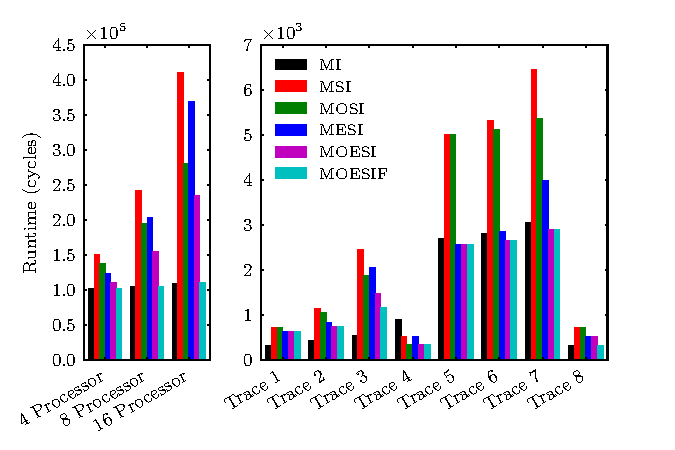
\includegraphics[width=\linewidth]{../runs/plots/runtime}
      \caption{Runtime (in clock cycles) of the various trace
        simulations using each cache coherency protocol. The longer
        validation runs are on the left plot, and the short traces are
        on the right.}
    \end{minipage}
  \end{figure}

  \begin{figure}[htbp]
    \label{fig:misses}
    \centering
    \begin{minipage}[t]{\figsize}
      \centering
      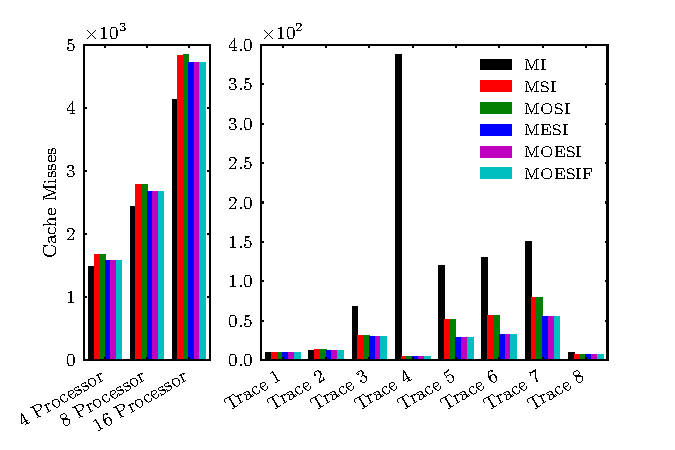
\includegraphics[width=\linewidth]{../runs/plots/misses}
      \caption{Number of cache misses during simulation of the various
        traces using each cache coherency protocol.}
    \end{minipage}
  \end{figure}

  \begin{figure}[htbp]
    \label{fig:transfers}
    \centering
    \begin{minipage}[t]{\figsize}
      \centering
      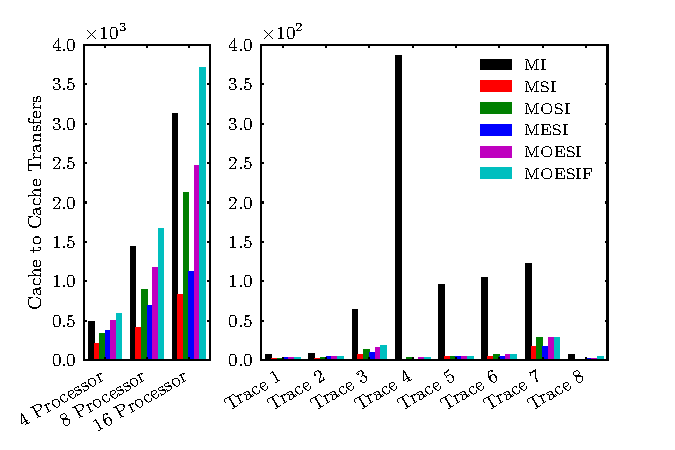
\includegraphics[width=\linewidth]{../runs/plots/transfers}
      \caption{Number of cache-to-cache transfers during simulation of
        the various traces using each cache coherency protocol.}
    \end{minipage}
  \end{figure}

  \begin{figure}[htbp]
    \label{fig:upgrades}
    \centering
    \begin{minipage}[t]{\figsize}
      \centering
      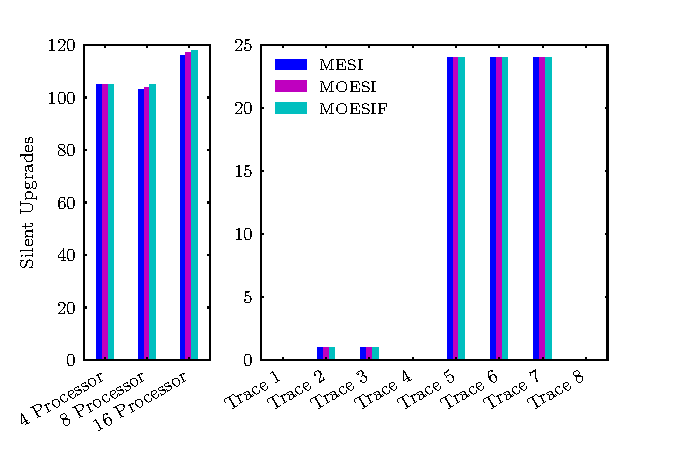
\includegraphics[width=\linewidth]{../runs/plots/upgrades}
      \caption{Number of silent upgrades to the modified state from
        the exclusive state during simulation of the various traces
        using each cache coherency protocol that contains an exclusive
        state.}
    \end{minipage}
  \end{figure}


\end{document}
